% Three-turn flowers pilot and terminal referee, grounded in flowers-debate-record.json.
\begingroup
\definecolor{fdInk}{HTML}{202830}
\definecolor{fdMuted}{HTML}{56616B}
\definecolor{fdGrey}{HTML}{C7D0D6}
\definecolor{fdBlue}{HTML}{246083}
\definecolor{fdGreen}{HTML}{23675B}
\definecolor{fdLight}{HTML}{F7F8FA}
\definecolor{fdBlueLight}{HTML}{EFF5F9}
\definecolor{fdGreenLight}{HTML}{EEF6F2}
\resizebox{\columnwidth}{!}{%
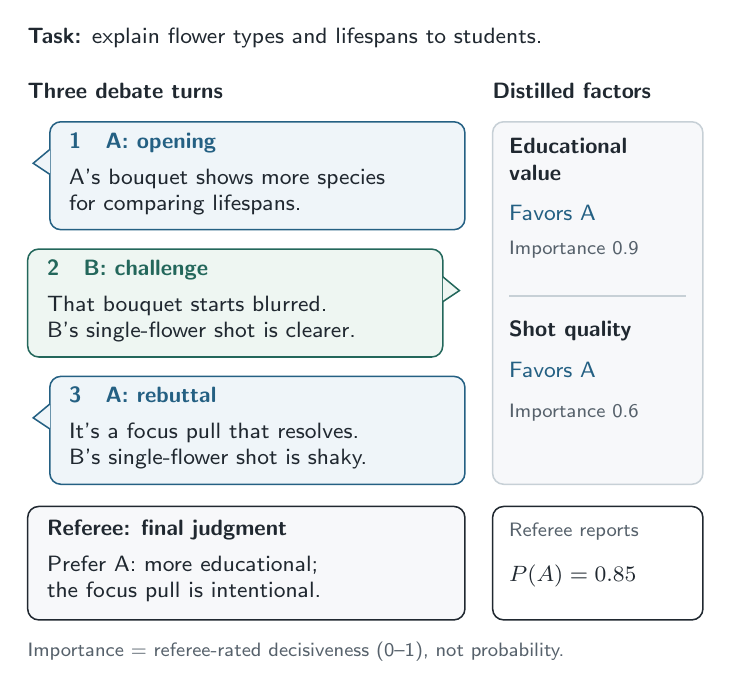
\begin{tikzpicture}[x=1pt,y=-1pt,
  fdtext/.style={anchor=north west,inner sep=0pt,outer sep=0pt,align=left,
    text=fdInk,font=\sffamily\fontsize{8}{9.4}\selectfont},
  fdhead/.style={fdtext,font=\sffamily\fontsize{8.2}{9.6}\selectfont\bfseries},
  fdsmall/.style={fdtext,text=fdMuted,font=\sffamily\fontsize{7}{8.2}\selectfont},
  fdcard/.style={line width=.55pt,rounded corners=4pt}
]
\path[use as bounding box] (0,0) rectangle (244,230);
\node[fdtext] at (0,0)
  {\textbf{Task:} explain flower types and lifespans to students.};
\node[fdhead] at (0,20) {Three debate turns};
\node[fdhead] at (168,20) {Distilled factors};
% Turn 1: A's opening.
\path[fdcard,draw=fdBlue,fill=fdBlueLight] (8,34) rectangle (158,73);
\path[draw=fdBlue,fill=fdBlueLight,line width=.55pt]
  (8,44) -- (2,49) -- (8,53);
\node[fdhead,text=fdBlue] at (15,38) {1\quad A: opening};
\node[fdtext,text width=136pt] at (15,51)
  {A's bouquet shows more species\newline for comparing lifespans.};
% Turn 2 explicitly challenges A's evidence.
\path[fdcard,draw=fdGreen,fill=fdGreenLight] (0,80) rectangle (150,119);
\path[draw=fdGreen,fill=fdGreenLight,line width=.55pt]
  (150,90) -- (156,95) -- (150,99);
\node[fdhead,text=fdGreen] at (7,84) {2\quad B: challenge};
\node[fdtext,text width=136pt] at (7,97)
  {That bouquet starts blurred.\newline B's single-flower shot is clearer.};
% Turn 3 answers the challenge rather than repeating the opening.
\path[fdcard,draw=fdBlue,fill=fdBlueLight] (8,126) rectangle (158,165);
\path[draw=fdBlue,fill=fdBlueLight,line width=.55pt]
  (8,136) -- (2,141) -- (8,145);
\node[fdhead,text=fdBlue] at (15,130) {3\quad A: rebuttal};
\node[fdtext,text width=136pt] at (15,143)
  {It's a focus pull that resolves.\newline B's single-flower shot is shaky.};
% Referee acts once after the debate, with no intervening questions.
\path[fdcard,draw=fdInk,fill=fdLight] (0,173) rectangle (158,214);
\node[fdhead] at (7,178) {Referee: final judgment};
\node[fdtext,text width=144pt] at (7,191)
  {Prefer A: more educational;\newline the focus pull is intentional.};
% Saved factor direction and decisiveness, not preference probabilities.
\path[fdcard,draw=fdGrey,fill=fdLight] (168,34) rectangle (244,165);
\node[fdhead,text width=64pt] at (174,40) {Educational\newline value};
\node[fdtext,text=fdBlue] at (174,64) {Favors A};
\node[fdsmall] at (174,77) {Importance 0.9};
\draw[draw=fdGrey,line width=.45pt] (174,97) -- (238,97);
\node[fdhead] at (174,106) {Shot quality};
\node[fdtext,text=fdBlue] at (174,121) {Favors A};
\node[fdsmall] at (174,136) {Importance 0.6};
\path[fdcard,draw=fdInk,fill=white] (168,173) rectangle (244,214);
\node[fdsmall] at (174,179) {Referee reports};
\node[fdhead] at (174,194) {$P(A)=0.85$};
\node[fdsmall] at (0,222)
  {Importance = referee-rated decisiveness (0--1), not probability.};
\end{tikzpicture}%
}
\endgroup
